\documentclass[11pt, a4paper]{article}

\usepackage{graphicx}
\usepackage[a4paper,top=3cm,bottom=2cm,left=2cm,right=2cm,marginparwidth=1.75cm]{geometry}
\usepackage[english]{babel}
\usepackage[utf8x]{inputenc}
\usepackage{subfig}
\usepackage{float}
\usepackage{amsmath}
\usepackage{amssymb}
\usepackage{mhchem}
\usepackage{hyperref}
\usepackage{tikz}
\usepackage{cancel}
\usepackage{bm}

\graphicspath{ {./images} }
\newcommand*{\qed}{\hfill\ensuremath{\quad\square}}%
\newcommand*{\rad}{\ensuremath{\,\text{rad}}}
\newcommand*{\R}{\ensuremath{\mathbb{R}}}
\newcommand*{\N}{\ensuremath{\mathbb{N}}}
\newcommand*{\C}{\ensuremath{\mathbb{C}}}
\renewcommand*{\Re}{\operatorname{Re}}
\renewcommand*{\Im}{\operatorname{Im}}
\renewcommand*{\epsilon}{\varepsilon}
\renewcommand*{\phi}{\varphi}
\renewcommand*{\d}{\text{d}}

\DeclareRobustCommand{\uvec}[1]{{%
  \ifcat\relax\noexpand#1%
    % it should be a Greek letter
    \bm{\hat{#1}}%
  \else
    \ifcsname uvec#1\endcsname
      \csname uvec#1\endcsname
    \else
      \bm{\hat{\mathbf{#1}}}%
     \fi
   \fi
}}

\makeatletter
\renewcommand*\env@matrix[1][*\c@MaxMatrixCols c]{%
  \hskip -\arraycolsep
  \let\@ifnextchar\new@ifnextchar
  \array{#1}}
\makeatother

\newtheorem{theorem}{Theorem}
\numberwithin{equation}{section}
\numberwithin{figure}{section}

%------------------------------------------------
%Templates for images and figures
% \begin{figure}[h]
%   \centering
%   \subfloat[caption 1]{{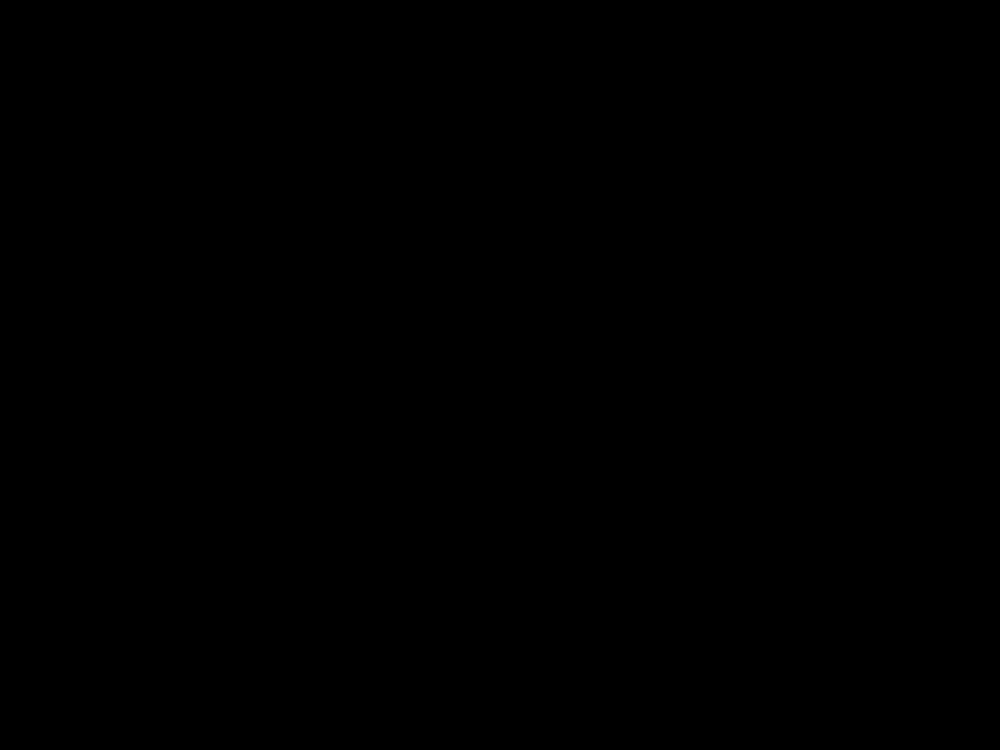
\includegraphics[width=30mm]{images/placeholder.png}}}%
%   \qquad
%   \subfloat[caption 2]{{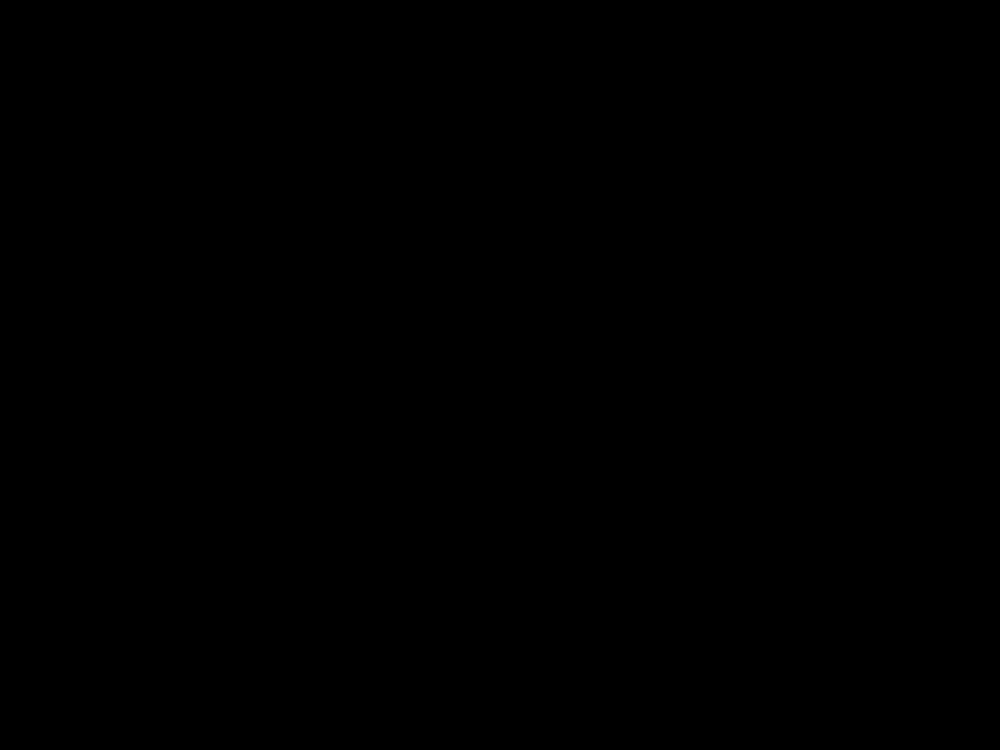
\includegraphics[width=30mm]{images/placeholder.png}}}%
%   \caption{Description}
% \end{figure}

% \begin{figure}[h]
%   \centerline{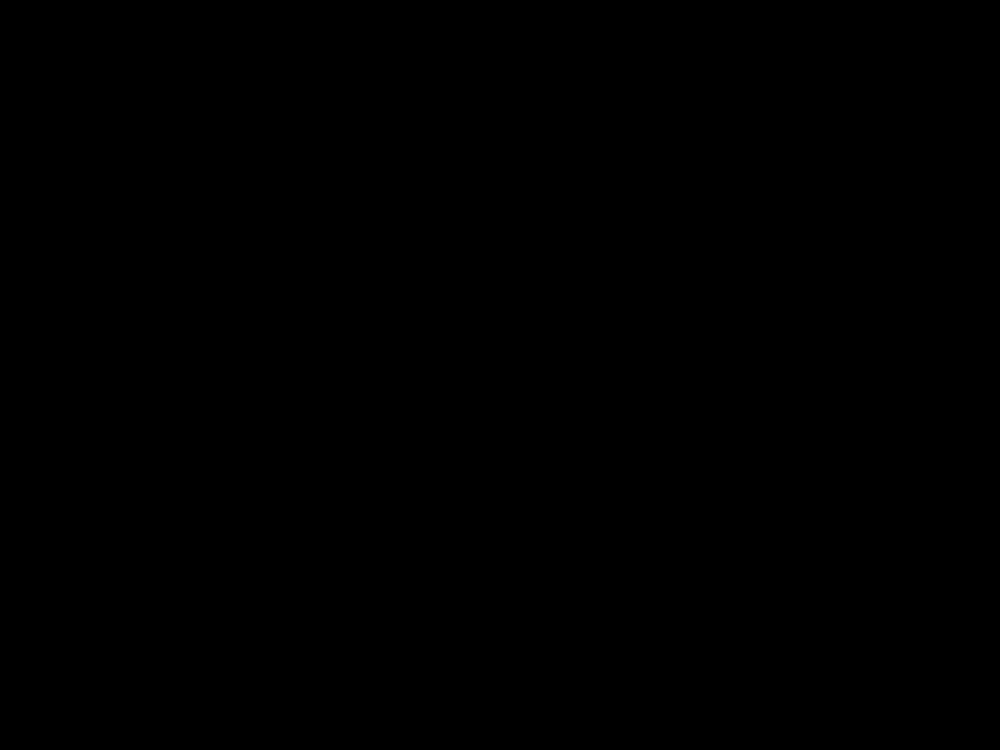
\includegraphics[width=50mm]{images/placeholder.png}}
%   \caption{Description}
% \end{figure}

%Template for a simple table 
%\begin{table}[h]
%   \caption{Description} %title of the table
%   \centering % centering table
%   \begin{tabular}{l rr} % creating three columns
%     \hline\hline %inserting double-line
%     & & \\ [0.5ex] % Insert half line vertical spacing
%     \hline % inserts single-line
%     & & \\ 
%     & & \\
%     & & \\
%     & & \\
%   \hline % inserts single-line
%   \end{tabular}
%   \label{tab:hresult}
% \end{table}
%-----------------------------------------------

\begin{document}
\setcounter{section}{5}

\section{Taylor and Maclaurin series}

\subsection{Introducing the Taylor and Maclaurin series}
Taylor series are a result of how power series function. Let $f(x)$ be some power series centered at the point $a$.
\begin{align}
  f(x) &= c_0 + c_1(x-a) + c_2(x-a)^2 + \cdots \notag\\
       &= \sum_{n=0}^\infty c_n(x-a)^n\;,\;|x-a| < R
\end{align}
When we evaluate this function at $x=a$ we find that $f(a)=c_0$. Now let's take the derrivative of $f(x)$ and evaluate it again at $x=a$:
\begin{equation*}
  \frac{\d f(x)}{\d x} = c_1 + 2c_2(x-a) + 3c_3(x-a)^2 + \cdots
\end{equation*}
Which gives $f'(a)=c_1$. We can keep repeating this for any $n$-th derrivative of $f(x)$. The pattern that starts to emerge when we do this for all terms of $f(x)$ up untill any $k$-th term will then be:
\begin{equation}
  f^{(k)}(x)=\sum_{n=k}^\infty n(n-1)\cdots(n-k+1)c_n(x-a)^{n-k}
\end{equation}
Which we can evaluate at $a$ to give:
\begin{equation}
  f^{(k)}(a) = k!c_k
\end{equation}
Rearranging this we find that:
\begin{equation}
  c_k = \frac{f^{(k)}(a)}{k!}
\end{equation}
Which means any $k$-th component of the power series $f(x)$ can be given as the $k$-th derrivative of the function eveluated at $a$ divided by $k!$. Subsituting this back into our original power series $f(x)$ with $k=n$ we get:
\begin{equation}
  f(x) = \sum_{n=0}^\infty \frac{f^{(n)}(a)}{n!}(x-a)^n
\end{equation}
In the special case that $a = 0$ we call this a Maclaurin series, which is nothing but a Taylor series centered at $x=0$.\\
\\
\underline{Example:} Determine the Maclaurin series of $f(x) = \exp(x)$.
\begin{align*}
  \forall\; &n\in\N\;f^{(n)}(x)=\exp(x) \Rightarrow f^{(n)}(0) = 1\\
  &\therefore \sum_{n=0}^\infty \frac{f^{(n)}(0)}{n!} x^n = \sum_{n=0}^\infty \frac{x^n}{n!}\quad \forall \;x\in\R
\end{align*}
When we evaluate this polynomial at $x=1$ we find that this polynomial gets closer and closer to a specific value for larger choices. When $n\to\infty$ we find that this eveluates exactly to:
\begin{equation*}
  \sum_{n=0}^\infty \frac{1}{n!} = e
\end{equation*} 
Where $e$ is Euler's number ($\approx 2.71828\cdots$). This means Euler's number is nothing but the exponetial function $\exp(x)$ eveluated at 1.\\
We can also eveluate this series with a more complex function: let $f(x)=\exp(2x)$. We tehn get:
\begin{align*}
  f^{(n)}(x) = 2^n\exp(2x) \Rightarrow &f^{(n)}(0) = 2^n \; \forall\,n\in\N\\
  &\therefore \exp(2x) = \sum_{n=0}^{\infty} \frac{2^nx^n}{n!}
\end{align*}
Which is the same result as what we would find for subsituting $2x$ for $x$ in the Maclaurin series for $\exp(x)$.


\subsection{Remainder terms of Taylor series and Taylor's theorem}
A complete Taylor series from 0 up untill $\infty$ can be split up in a partial sum of the Taylor series and the remainder terms of the series. This looks a bit like:
\begin{equation}
  \sum_{n=0}^{\infty} T_n = \sum_{n=0}^{N} T_n + \sum_{n=N+1}^{\infty} T_n
\end{equation}
Where $\sum_{n=N+1}^{\infty} T_n = R_n$ which is the remainder term of the Taylor series. Subistuting back in the definition of a Taylor series we get:
\begin{equation}
  \sum_{n=0}^\infty \frac{f^{(n)}(a)}{n!}(x-a)^n = \sum_{n=0}^N \frac{f^{(n)}(a)}{n!}(x-a)^n + \sum_{n=N+1}^\infty \frac{f^{(n)}(a)}{n!}(x-a)^n
\end{equation}
Taylor's theorem is a way of quantifying the remainder term of a Taylor series:
\begin{gather}
  |f^{(n+1)}(x)|\leq M\;, \left(a-d\leq x \leq a+d\right) \rightarrow \,x\in[a-d,\,a+d]: \notag\\
  |R_n(x)| = |f(x) - T(x)| \leq \frac{M}{(n+1)!}|x-a|^{(n+1)} \leq \frac{Md^{(n+1)}}{(n+1)!}
\end{gather}


\subsection{Taylor series of trigonometric functions}
In this section we will analyse the Taylor series of a trigonometric function by studying $f(x) = \sin(x)$:
\begin{align}
  \begin{cases}
    f(x) = \sin(x) &\Rightarrow f(0) = 0\\
    f'(x) = \cos(x) &\Rightarrow f'(0) = 1\\
    f''(x) = -\sin(x) &\Rightarrow f''(0) = 0\\
    f'''(x) = -\cos(x) &\Rightarrow f'''(0) = -1\\
    f''''(x) = \sin(x) &\Rightarrow f''''(0) = 0\\
    \vdots
  \end{cases}
\end{align}
By filling this into the Maclaurin series of $f(x)$ we find that:
\begin{gather}
  x - \frac{x^3}{3!} + \frac{x^5}{5!} - \frac{x^7}{7!} + \cdots = \sum_{n=0}^{\infty} (-1)^n \frac{x^{2n+1}}{(2n+1)!}\notag\\
  \therefore \sin(x) = \sum_{n=0}^{\infty} (-1)^n\frac{x^{2n+1}}{(2n+1)!}
\end{gather}
From this we can also derrive the Taylor series of $\cos(x)$ since it's nothing but the first derriavtive of the Taylor series of $\sin(x)$ we find that:
\begin{align}
  \forall x \in \R,\, \cos(x) &= \frac{\d(\sin(x))}{\d x} \notag\\
                              &= \sum_{n=0}^{\infty} \frac{\d}{\d x} \left( (-1)^n\frac{x^{2n+1}}{(2n+1)!} \right) \notag\\
                              &= \sum_{n=0}^{\infty} (-1)^n\frac{x^{2n}}{(2n)!}
\end{align}



\subsection{List of common Taylor series}
\begin{itemize}
  \item [] $\exp(x) = \sum_{n=0}^{\infty} \frac{x^n}{n!} \quad x\in\R$
  \item [] $\sin(x) = \sum_{n=0}^{\infty} (-1)^n \frac{x^{2n+1}}{(2n+1)!} \quad x\in\R$
  \item [] $\cos(x) = \sum_{n=0}^{\infty} (-1)^n \frac{x^{2n}}{(2n)!} \quad x\in\R$
  \item [] $\ln(1+x) = \sum_{n=0}^{\infty} (-1)^{n+1} \frac{x^n}{n} \quad x \in (-1, 1]$
  \item [] $\arctan(x) = \sum_{n=0}^{\infty} (-1)^n \frac{x^{2n+1}}{2n+1} \quad x\in(-1, 1)$
\end{itemize}
\end{document}